\chapter{Methodology}
\section{Outline}
This section will look into the mathematical designs for the Stewart platform, considerations for the force sensor and the velocity measurement within the wind tunnel. It will finally look into the design of a human machine interface that will be used to control the Stewart platform,  obtain the measurements and display results.

\section{Design of Stewart Platform}
This section deals with: design considerations, position, velocity and acceleration analysis of the Stewart platform.
\subsection{Design Considerations}
\begin{enumerate}
\item When the controllable axes are active, the platform must be controlled in six degrees of motion.
\item When the controllable members are stationary, the
platform must have a corresponding fixed position.
\item The design parameters for consideration are: mobile platform radius, height of the platform and angle between adjacent joints of mobile platform and base plate.
\item The mechanism should be lightweight.
\item Velocity and position control of the mechanism should be easy to achieve.
\end{enumerate}
\subsection{Kinematic Analysis - Rotational matrix}
Euler angles are utilized to obtain rotational matrix for the moving platform of the Stewart platform mechanism. The rotational matrix is represented as follows \cite{csumnu2017simulation}:
\begin{equation}
 R_{P}^B = R_{Z}(\gamma)*R_{Y}(\beta)*R_{X}(\alpha)
\end{equation}
Where $\gamma, \beta, \alpha$ - angles of rotation about the z-, y- and x-axis respectively.

In matrix form:
\[ R_{P}^B =
 \begin{bmatrix}
 c\beta c\gamma & s\alpha s\beta c\gamma - c\alpha s\gamma & c\alpha s\beta c\gamma + s\alpha s\gamma\\
 c\beta s\gamma & s\alpha s\beta s\gamma + c\alpha c\gamma & c\alpha s\beta s\gamma - s\alpha c\gamma\\
 -s\beta & s\alpha c\beta & c\alpha c\beta  
 \end{bmatrix}
\]
Generalized coordinate position and velocity vector of the moving platform is represented below \cite{csumnu2017simulation}:
\[
q=
\begin{bmatrix}
tx & ty & tz & \alpha & \beta & \gamma
\end{bmatrix}^\top
\]
\[
\dot{q}=
\begin{bmatrix}
\dot{tx} & \dot{ty} & \dot{tz} & \dot{\alpha} & \dot{\beta} & \dot{\gamma}
\end{bmatrix}^\top
\]
Transformation of angular velocity of moving platform to the base frame can be done using Euler angles \cite{csumnu2017simulation}:
\[
\omega =
\begin{bmatrix}
1 & 0 & s\beta \\
0 & c\alpha & -s\alpha c\beta \\
0 & s\alpha & c\alpha c\beta 
\end{bmatrix}
\begin{bmatrix}
\dot{\alpha} \\
\dot{\beta}\\
\dot{\gamma}
\end{bmatrix}
\]
Acceleration of the moving platform is obtained by differentiating the velocity of the moving platform with respect to time:
\[
\dot{\omega} =
\begin{bmatrix}
1 & 0 & s\beta \\
0 & c\alpha & -s\alpha c\beta \\
0 & s\alpha & c\alpha c\alpha c\beta 
\end{bmatrix}
\begin{bmatrix}
\ddot{\alpha} \\
\ddot{\beta}\\
\ddot{\gamma}
\end{bmatrix}
+
\begin{bmatrix}
0 & 0 & \dot{\beta}c\beta \\
0 & \dot{\alpha} s\alpha & -\dot{\alpha} c\alpha c\beta + s\alpha \dot{\beta} s\beta \\
0 & \dot{\alpha}c\alpha & -\dot{\alpha}s\alpha c\beta - c\alpha \dot{\beta}s\beta
\end{bmatrix}
\begin{bmatrix}
\dot{\alpha} \\
\dot{\beta}\\
\dot{\gamma}
\end{bmatrix}
\]
\subsection{Inverse Kinematic Analysis}
Inverse kinematic analysis is used to determine the length of the legs according to planned trajectories of the moving platform position. In order to consider the length of the leg of a Stewart platform, closed-loop of one leg is used as shown in figure 3.1. Using this closed-form representation, the leg
vector with respect to base platform can be obtained as follows \cite{csumnu2017simulation}:
\begin{equation}
\label{eqn}
L_{i} = q_{i}^{B} - b_{i}
\end{equation}
The position vector of ith upper junction point with respect to the base frame is given by the following;
\begin{equation}
\label{eqn}
q_{i}^{B} = t + R_{p}^{B} * q_{i}^{p}
\end{equation}
\begin{center}
	\begin{figure}[!h]
	\centering
	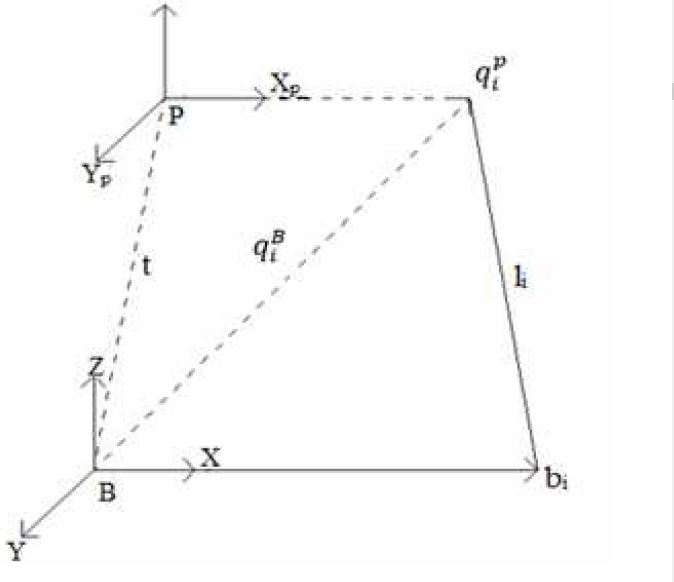
\includegraphics[width=0.6\linewidth]{Figures/Fig12}
	\caption[Closed-loop representation]{Closed-loop representation of one leg of the Stewart Platform \cite{csumnu2017simulation}}
	\end{figure}
\end{center}
Then the length of the ith leg can be acquired as follows:
\newpage
\begin{equation}
\label{eqn}
l_{i}^2 = (a_{x} * r_{p} * c_{i} + b_{x}*r_{p}*s_{i}
+ t_{x}-r_{b}*c_{i})^2 \\+ (a_{y}*r_{p}*c_{i} + b_{y}*r_{p}*s_{i} + t_{y}-r_{b}*s_{i})^2 \\+ (a_{z}*r_{p}*c_{i}+b_{z}*r_{p}*s_{i}+t_{z})^2
\end{equation}
\subsection{Inverse Velocity Analysis}
Inverse Jacobian matrix can be used to perform inverse velocity analysis of the Stewart
platform. Inverse Jacobian matrix describes relation between velocity of the moving platform and the leg velocity.

Inverse Jacobian matrix for a 6-DOF Stewart Platform
\cite{csumnu2017simulation}:
\[ J^-1 =
\begin{bmatrix}
u_{1}^{T} & (R_{P}^{B}q_{1}^{B} * u_{1})^T\\
u_{2}^{T} & (R_{P}^{B}q_{2}^{B} * u_{2})^T\\
u_{3}^{T} & (R_{P}^{B}q_{3}^{B} * u_{3})^T\\
u_{4}^{T} & (R_{P}^{B}q_{4}^{B} * u_{4})^T\\
u_{5}^{T} & (R_{P}^{B}q_{5}^{B} * u_{5})^T\\
u_{6}^{T} & (R_{P}^{B}q_{6}^{B} * u_{6})^T
\end{bmatrix}
\]
\subsection{PID Control of the Stewart Platform}
The controller will consist of two sections:
\begin{enumerate}
\item The leg trajectory - will be used to generate the desired leg lengths for each time step.
\item The Controller.
\end{enumerate}  The following equation will be used to calculate the leg lengths for each leg 
\cite{smith2002creating}:
\begin{equation}
\label{eqn}
((R*p_{t,i} + p)-p_{b,j}))- l_{n,i}
\end{equation}
where R is the rotation matrix relating the top plate orientation with respect to the bottom plate, $P_{t,i}$ is the attachment point of leg i in the top plate with respect to the top plate coordinate system, P is the position of the top plate with respect to the bottom plate, $P_{b,i}$ is the attachment point of leg i in the bottom plate with respect to the bottom plate coordinate system, and $ln,i$ is the nominal length of leg i. 

Proportional-integral-derivative (PID) control will be used to control the Stewart platform. A dynamic model of the system, such as the one shown in figure 3.2, will be implemented in MatLab/Simulink.
\begin{center}
	\begin{figure}[!h]
	\centering
	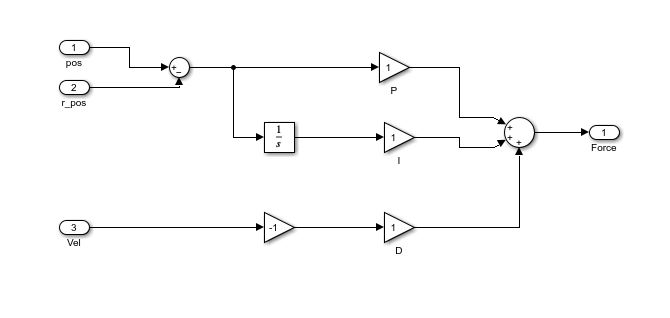
\includegraphics{Figures/Fig13}
	\caption[PID Controller]{Simple Low-level PID Controller}
	\end{figure}
\end{center}
\section{Design of the Force Sensor}
The force sensor module will be used to measure the force and moments from the aerodynamic loads applied on model being tested in the wind tunnel. The forces to be measured are the drag, lift and thrust as well as associated moments. For this subsystem two possible conceptual designs are to be considered:
\begin{itemize}
\item External force sensor
\item Stewart Platform as a force sensor
\end{itemize}
\subsection{External Force Sensor}
In this case it would require at least 3 orthogonally positioned load cells measuring each force component. Each load cell would be mechanically linked to the model such that forces experienced on each axis are measured by each load cell. 
\begin{center}
	\begin{figure}[!h]
		\centering
		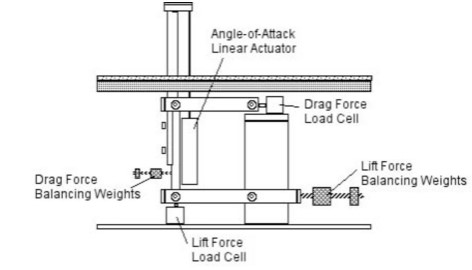
\includegraphics{Figures/modBal}
		\caption[Diagram of a force balance]{Diagram of a force balance \cite{post_force_2010}}
	\end{figure}
\end{center}
This configuration is however bulky by requiring an additional external system for force measurements in addition to the stewart platform for positioning the model. This is however complemented by the simplicity in calibration of the load cells and does not require a complex force transformation matrix and other issues with force amplification created by the use of an integrated system.
\subsection{Stewart Platform as a force sensor}
In this configuration the stewart platform legs are used as force sensors by attaching strain gauges in the legs of platform. Similar work has been done by \cite{ferreira2015design} without the use of actuators as is proposed in this project. Using the stewart platform as a force sensor requires the actuators to be locked with zero degrees of freedom.

Four strain gauges are required for each leg for a full wheatstone bridge configuration. 
\begin{center}
	\begin{figure}[!h]
		\centering
		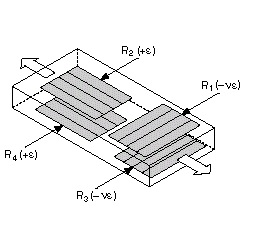
\includegraphics{Figures/loadConf}
		\caption[Strain Gauge Configuration]{Strain Gauge Configuration \cite{noauthor_measuring_nodate}}
	\end{figure}
\end{center}
In this case as shown in the figure the load cells are able to measure the axial strain on each leg. R1 and R3 are active strain gauges measuring the compressive Poisson effect (–νe). R2 and R4 are active strain gages measuring the tensile strain (+e). The output generated from the wheatstone bridge is then amplified and read to determine the strain on each leg.

\paragraph{Force measurement Circuit}
The output excitation of the wheatstone brisge needs to be amplified as it results in low outputs. An analog to digital converter is also reuiqred fot the analog to digital conveter. Some considerable options are the hx711 or the AD7193 converters which may be used as digital to analog converters. The AD7193 is designed for high precision and has a delta sigma filter to remove noise from measurements. 

The connection of the AD7193 to the microcontroller will be via Serial Peripheral Interface (SPI). the configuration is as shown in the figure:
\begin{center}
\begin{figure}
\centering
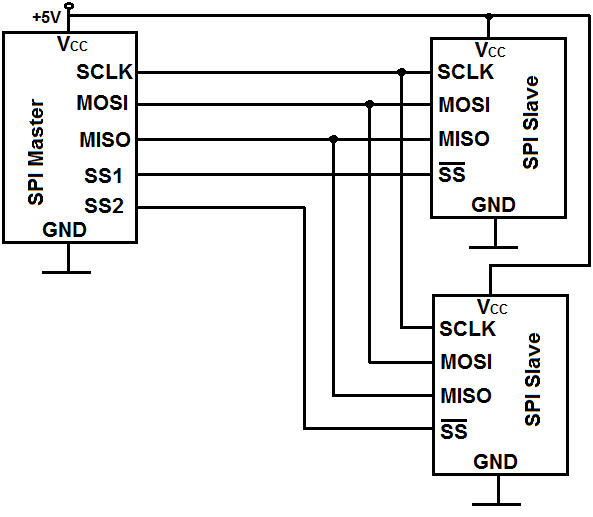
\includegraphics[width=0.55\linewidth]{Figures/SPI}
\caption[SPI configuration]{SPI configuration}
\end{figure}
\end{center}
In this configuration the when the chip select of an amplifier is set to low, the microcontroller is able to obtain data from that strain gauge. This configuration allows for a four wire interface to connect to six strain gauge sensors and obtain measurements.

\paragraph{Force transformation matrix} 
In such a case the forces experienced at the top of the platform are distributed between the 6 legs and as result, a force transformation matrix is required to resolve the forces apllied on each axis as measured by each load cell on each leg. 

If the platform is acted upon by an external wrench {$\vec{F}_e, \vec{M}_e$}, for static equilibrium of the body, the external wrench is statically balanced by the six leg forces of the stewart platform. Representing the unit vector $\hat{I}_i$ along the i-th leg with respect to B, the leg force is given  by $\hat{I}_if_i$. Considering the force equilibrium of the platform along  three mutually perpendicular directions in B(XYZ), the following force equations can be obtained as in \cite{dwarakanath_design_2001}:

$(F_e)_x = f_1I_{1x} + f_2I_{2x} + f_3I_{3x} + f_4I_{4x} + f_5I_{5x} + f_6I_{6x}$

$(F_e)_y = f_1I_{1y} + f_2I_{2y} + f_3I_{3y} + f_4I_{4y} + f_5I_{5y} + f_6I_{6y}$

$(F_e)_z = f_1I_{1z} + f_2I_{2z} + f_3I_{3z} + f_4I_{4z} + f_5I_{5z} + f_6I_{6z}$

where $(F_e)_x$, $(F_e)_y$ and $(F_e)_z$ are the external forces on the platform along three mutually perpendicular directions x, y and z of the frame B, respectively.

The moment due to the forces $\hat{I}_if_i$ about the origin of B is $(\vec{b}_i x \hat{I}_i)f_i$. Considering the moment equilibrium about x, y and z axes of B, the following moment equations can be obtained as in \cite{dwarakanath_design_2001}:

$(M_e)_x = f_1(\vec{b}_1 x \hat{I}_1)_x + f_2(\vec{b}_2 x \hat{I}_2)_x + f_3(\vec{b}_3 x \hat{I}_3)_x + f_4(\vec{b}_4 x \hat{I}_4)_x + f_5(\vec{b}_5 x \hat{I}_5)_x + f_6(\vec{b}_6 x \hat{I}_6)_x$

}$(M_e)_y = f_1(\vec{b}_1 x \hat{I}_1)_y + f_2(\vec{b}_2 x \hat{I}_2)_y + f_3(\vec{b}_3 x \hat{I}_3)_y + f_4(\vec{b}_4 x \hat{I}_4)_y + f_5(\vec{b}_5 x \hat{I}_5)_y + f_6(\vec{b}_6 x \hat{I}_6)_y$

$(M_e)_z = f_1(\vec{b}_1 x \hat{I}_1)_z + f_2(\vec{b}_2 x \hat{I}_2)_z + f_3(\vec{b}_3 x \hat{I}_3)_z + f_4(\vec{b}_4 x \hat{I}_4)_z + f_5(\vec{b}_5 x \hat{I}_5)_z + f_6(\vec{b}_6 x \hat{I}_6)_z$

where $(M_e)_x$, $(M_e)_y$ and $(M_e)_z$ are the external moments on the platform  about the three coordinate axes of B. Combining the equations the relationship between the external wrench and the forces experienced by the legs can be expressed as follows:
$$
\begin{Bmatrix}
\vec{F}_e \\
\vec{M}_e \\
\end{Bmatrix} = [H]\{F\}
$$

\section{Velocity Measurement}
An important part in wind tunnel measurements is the measure of pressure at specific points in the wind tunnel and computing the corresponding air speed. This is achieved by the use of a pitot probe. 
\begin{center}
\begin{figure}
\centering
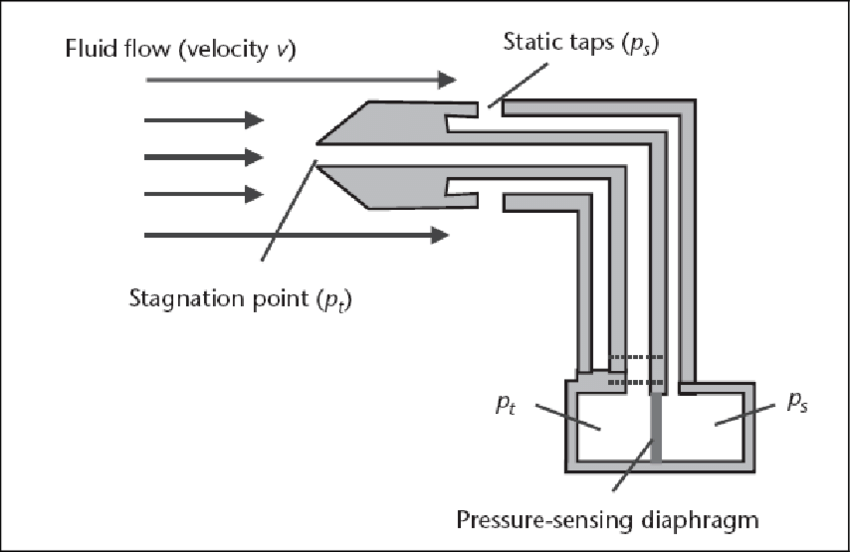
\includegraphics[width=0.6\linewidth]{Figures/pitot}
\caption[Pitot-static tube]{Pitot-static tube \cite{noauthor_wind_nodate}}
\end{figure}
\end{center}
The equation relates the speed of the fluid at a point to both the mass density of the fluid and the pressures at the same point in the flow field. For steady flow of an incompressible fluid for which viscosity can be neglected, the fundamental equation has the form:

$$ v = \sqrt{\frac{2(P_{0} - P)}{\rho}}$$

Where V is the speed of the fluid, P0 is the total, also called the stagnation, pressure at that point of measurement, and p is the static pressure at the same point.

Three pitot probes are to be used in the wind tunnel, these are in the test section, intake and dissuser sections.

\section{Design of Human Machine Interface}
The purpose of the interface is to enable control of the platform position as well as to obtain measured data from the strain gauges and pitot tubes. 
The general layout is as shown in the figure below:
\begin{center}
\begin{figure}
\centering
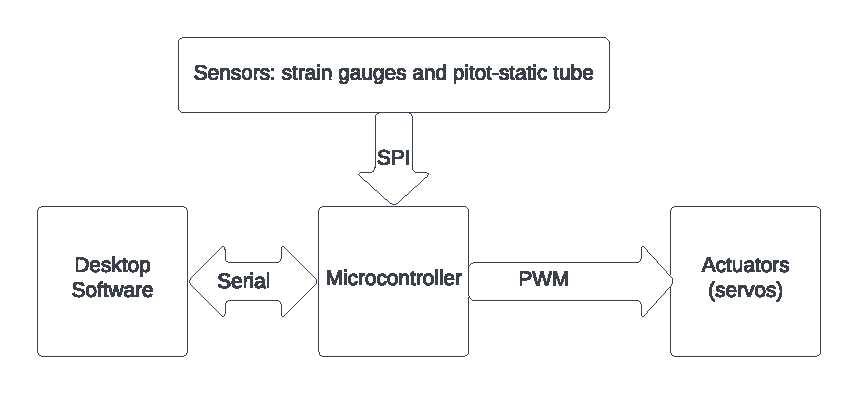
\includegraphics{Figures/interface}
\caption[Human Machine Interface]{Human Machine Interface}
\end{figure}
\end{center}

The primary interface between the microcontroller is via serial interface by use of USB. This is used due to wide availability and integration on many personal computers. Serial communication allows for bidirectional transfer of information thus allowing for both control input and output of measured values. The interface is to enable the abstraction of data aquisition and actuator control to a simple interaction with buttons and other visual interfaces available in a computer program.

The decoupling of the microcontroller and the program to be hosted on the desktop allows for advanced data processing such as application of filters and resolving measurements into useable information. It also allows for the use of more powerful processor and high level programmming languages to more effectively perform complex calculations without taking a toll the sensor samping rate that would occur with onboard processing in the microcontroller.
\begin{center}
	\begin{figure}[!h]
	\centering
	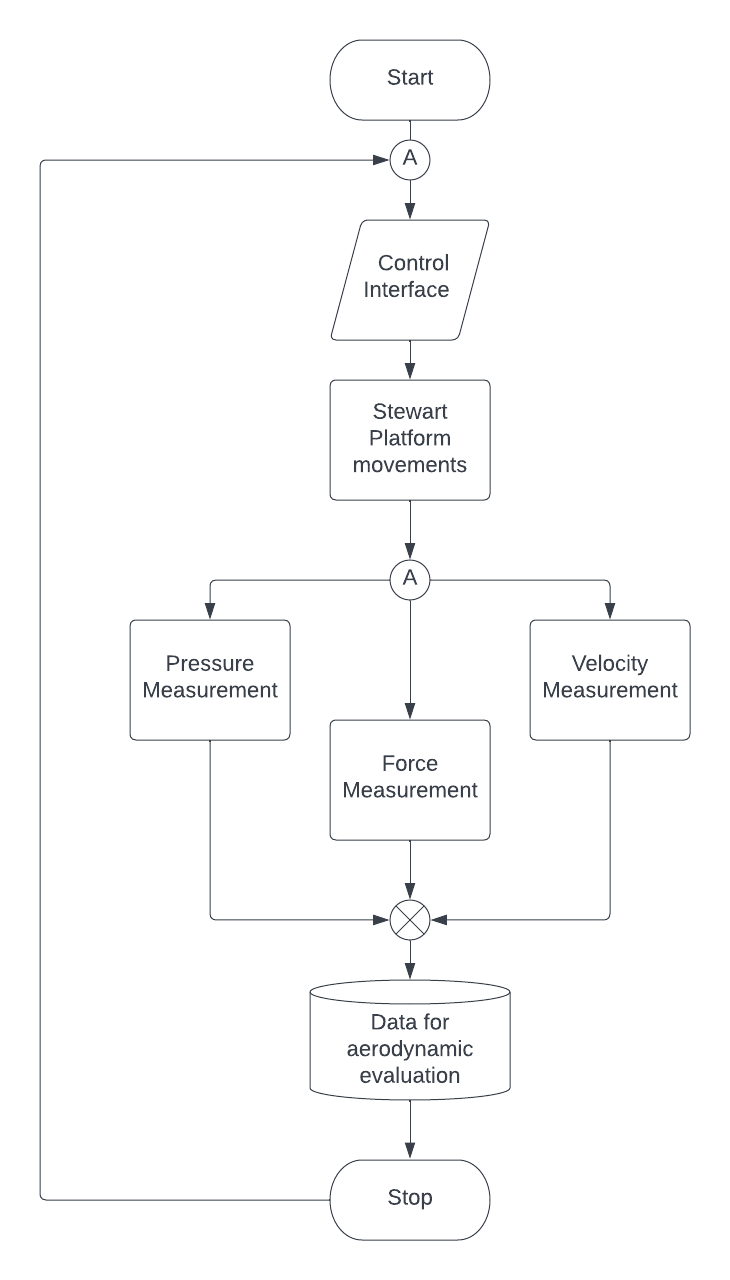
\includegraphics[width=0.7\linewidth]{Figures/Fig14}
	\caption[Control Algorithm]{Control Algorithm for the Stewart Platform with Force Measurement}
	\end{figure}
\end{center}